\documentclass[8pt,a4paper,compress]{beamer}

\usepackage{/home/siyer/lib/slides}

\title{Recursion}
\date{}

\begin{document}
\begin{frame}
\vfill
\titlepage
\end{frame}

\begin{frame}
\frametitle{Outline}
\tableofcontents
\end{frame}

\section{What is Recursion?}
\begin{frame}[fragile]
\pause

A recursive function is a function that calls itself and meets the following conditions
\begin{itemize}
\item Has a base case
\item Addresses subproblems that are smaller in some sense
\item Does not address subproblems that overlap
\end{itemize}

\pause
\bigskip

Recursive programming is directly related to mathematical induction, a technique for proving facts about discrete functions, such as $1 + 2 + 3 + \dots + n = \frac{n(n+1)}{2}$
\end{frame}

\section{Examples}
\begin{frame}[fragile]
\pause

Recursive definition of the factorial function $N!$ 
\[
N! = \begin{dcases*}
N(N-1)! & if $N > 0$, and \\
1       & if $N=0$
\end{dcases*}
\]

\pause
\bigskip

Implementation of $N!$ in Python

\begin{lstlisting}[language=Python]
def factorial(N):
    if N == 0:
        return 1
    return N * factorial(N - 1)
\end{lstlisting}

\pause
\bigskip

Call trace for \lstinline{factorial(5)}
\begin{lstlisting}[language={}]
factorial(5)
  factorial(4)
    factorial(3)
      factorial(2)
        factorial(1)
          factorial(0)
            return 1
          return 1 * 1 = 1            
        return 2 * 1 = 2
      return 3 * 2 = 6
    return 4 * 6 = 24
  return 5 * 24 = 120
\end{lstlisting}
\end{frame}

\begin{frame}[fragile]
\pause

Recursive definition of the $n$th harmonic number $H_n$
\[
H_n = \begin{dcases*}
\frac{1}{n} + H_{n-1} & if $n > 1$, and \\
1       & if $n=1$
\end{dcases*}
\]

\pause
\bigskip

Implementation of $H_n$ in Python
 
\begin{lstlisting}[language=Python]
def harmonic(n):
    if n == 1:
        return 1
    return 1 / n + harmonic(n - 1)
\end{lstlisting}

\pause
\bigskip

Call trace for \lstinline{harmonic(5)}
\begin{lstlisting}[language={}]
harmonic(5)
  harmonic(4)
    harmonic(3)
      harmonic(2)
        harmonic(1)
          return 1
        return 1 / 2 + 1 = 1.5
      return 1 / 3 + 1.5 = 1.8333333333333333
    return 1 / 4 + 1.8333333333333333 = 2.083333333333333
  return 1 / 5 + 2.083333333333333 = 2.283333333333333
\end{lstlisting}
\end{frame}

\begin{frame}[fragile]
\pause

Recursive definition of Euclid's algorithm for computing the greatest common divisor (gcd) of $p$ and $q$
\[
\text{gcd}(p, q) = \begin{dcases*}
\text{gcd}(q, p \bmod q) & if $q \neq 0$, and \\
p       & if $q = 0$
\end{dcases*}
\]

\pause
\bigskip

Implementation of $\text{gcd}(p, q)$ in Python

\begin{lstlisting}[language=Python]
def gcd(p, q):
    return p if q == 0 else gcd(q, p % q) 
\end{lstlisting}

\pause
\bigskip

Call trace for \lstinline{gcd(1440, 408)}

\begin{lstlisting}[language={}]
gcd(1440, 408)
  gcd(408, 216)
    gcd(216, 192)
      gcd(192, 24)
        gcd(24, 0)
          return 24
        return 24
      return 24
    return 24
  return 24
\end{lstlisting}
\end{frame}

\begin{frame}[fragile]
\pause

\begin{framed}
\tiny towersofhanoi.py: Accept integer $n$ as a command-line argument. Write to standard output instructions to move $n$ Towers of Hanoi disks to the left.
\end{framed}

\begin{minipage}{200pt}
\begin{lstlisting}[language=Python]
import stdio
import sys

def moves(n, left):
    if n == 0:
        return
    moves(n - 1, not left)
    if left:
        stdio.writeln(str(n) + ' left')
    else:
        stdio.writeln(str(n) + ' right')
    moves(n - 1, not left)

def main():
    n = int(sys.argv[1])
    moves(n, True)

if __name__ == '__main__':
    main()
\end{lstlisting}

\pause

\begin{lstlisting}[language={}]
$ python3 towersofhanoi.py 3
1 left
2 right
1 left
3 left
1 left
2 right
1 left
\end{lstlisting}
\end{minipage}
\begin{minipage}{100pt}
\visible<2->{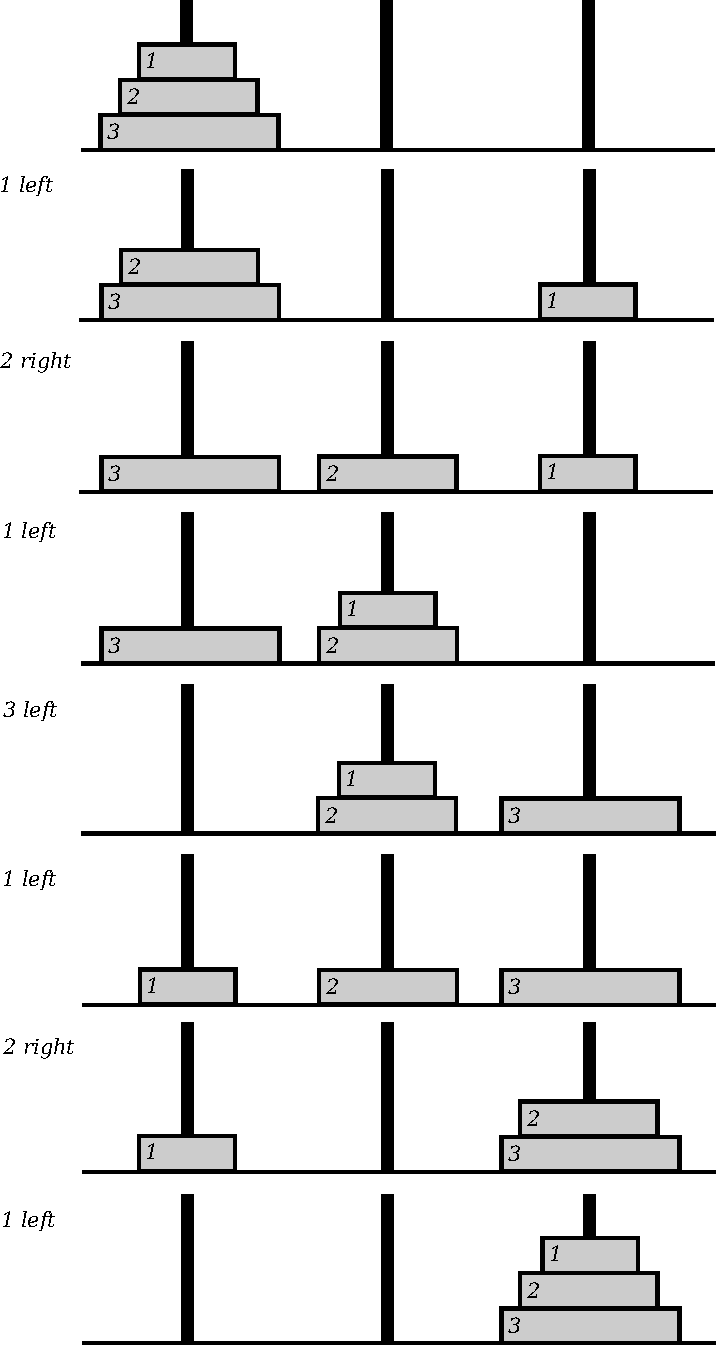
\includegraphics[scale=0.3]{figures/hanoi.pdf}}
\end{minipage}
\end{frame}

\begin{frame}[fragile]
\pause

Call trace for \lstinline{moves(3, True)}

\begin{lstlisting}[language={}]
moves(3, True)
  moves(2, False)
    moves(1, True)
      1 left
    2 right
    moves(1, True)
      1 left
  3 left
  moves(2, False)
    moves(1, True)
      1 left
    2 right
    moves(1, True)
      1 left
\end{lstlisting}

\pause

\begin{lstlisting}[language={}]
$ python3 towersofhanoi.py 4
1 right
2 left
1 right
3 right
1 right
2 left
1 right
4 left
1 right
2 left
1 right
3 right
1 right
2 left
1 right
\end{lstlisting}
\end{frame}

\begin{frame}[fragile]
\pause

Call trace for \lstinline{moves(4, True)}

\begin{lstlisting}[language={}]
moves(4, True)
  moves(3, False)
    moves(2, True)
      moves(1, False)
        1 right
      2 left
      moves(1, False)
        1 right
    3 right
    moves(2, True)
      moves(1, False)
        1 right
      2 left
      moves(1, False)
        1 right
  4 left
  moves(3, False)
    moves(2, True)
      moves(1, False)
        1 right
      2 left
      moves(1, False)
        1 right
    3 right
    moves(2, True)
      moves(1, False)
        1 right
      2 left
      moves(1, False)
        1 right
\end{lstlisting}
\end{frame}

\begin{frame}[fragile]
\pause

\begin{framed}
\tiny htree.py: Accept integer $n$ as a command-line argument. Draw a level $n$ H-tree centered at $(.5, .5)$ with lines of length $.5$.
\end{framed}

\begin{lstlisting}[language=Python]
import stddraw
import sys

def draw(n, lineLength, x, y):
    if n == 0:
        return
    x0 = x - lineLength / 2
    x1 = x + lineLength / 2
    y0 = y - lineLength / 2
    y1 = y + lineLength / 2
    stddraw.line(x0, y, x1, y)
    stddraw.line(x0, y0, x0, y1)
    stddraw.line(x1, y0, x1, y1)
    draw(n - 1, lineLength / 2, x0, y0)
    draw(n - 1, lineLength / 2, x0, y1)
    draw(n - 1, lineLength / 2, x1, y0)
    draw(n - 1, lineLength / 2, x1, y1)

def main():
    n = int(sys.argv[1])
    stddraw.setPenRadius(0.0)
    draw(n, .5, .5, .5)
    stddraw.show()

if __name__ == '__main__':
    main()
\end{lstlisting}
\end{frame}

\begin{frame}[fragile]
\pause

\begin{minipage}{160pt}
\begin{lstlisting}[language={}]
$ python3 htree.py 1
\end{lstlisting}
\end{minipage}%
\begin{minipage}{140pt}
\hfill \visible<2->{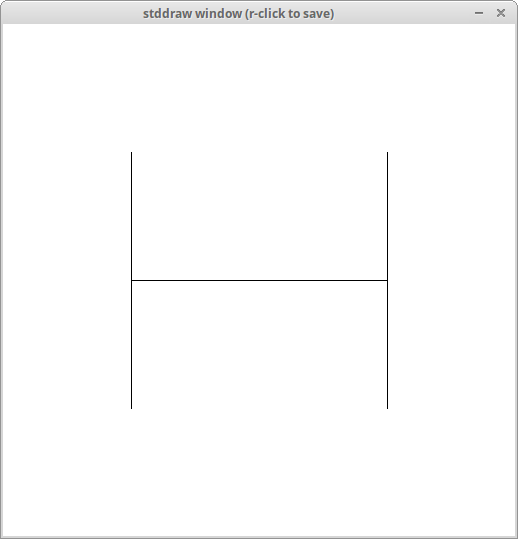
\includegraphics[scale=0.15]{figures/htree1.png}}
\end{minipage}

\pause
\smallskip

\begin{minipage}{160pt}
\begin{lstlisting}[language={}]
$ python3 htree.py 3
\end{lstlisting}
\end{minipage}%
\begin{minipage}{140pt}
\hfill \visible<3->{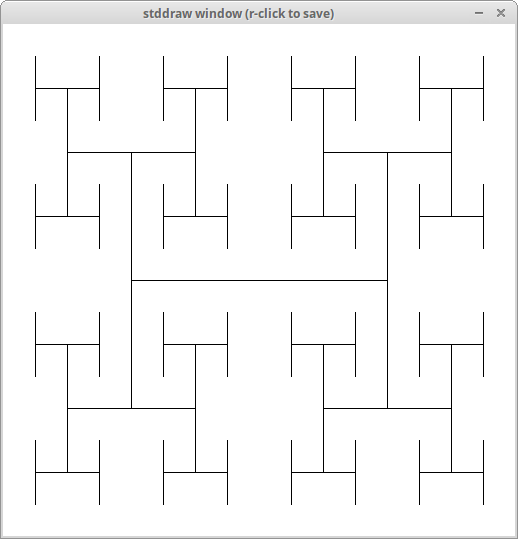
\includegraphics[scale=0.15]{figures/htree2.png}}
\end{minipage}

\pause
\smallskip

\begin{minipage}{160pt}
\begin{lstlisting}[language={}]
$ python3 htree.py 5
\end{lstlisting}
\end{minipage}%
\begin{minipage}{140pt}
\hfill \visible<4->{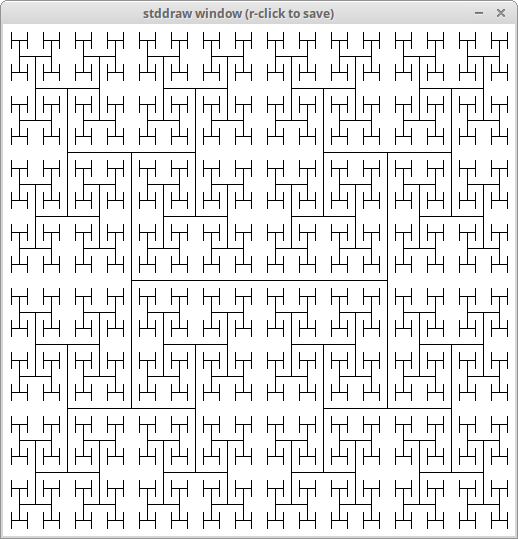
\includegraphics[scale=0.15]{figures/htree3.png}}
\end{minipage}
\end{frame}

\begin{frame}[fragile]
\pause

\begin{framed}
\tiny brownian.py: Accept a Hurst exponent as a command-line argument. Use the Hurst exponent to compute a scale factor. Draw a Brownian bridge from $(0, .5)$ to $(1.0, .5)$ with variance $.01$ and that scale factor.
\end{framed}

\begin{lstlisting}[language=Python]
import math
import stddraw
import stdrandom
import sys

def curve(x0, y0, x1, y1, variance, scaleFactor):
    if (x1 - x0) < .01:
        stddraw.line(x0, y0, x1, y1)
        return
    xm = (x0 + x1) / 2.0
    ym = (y0 + y1) / 2.0
    delta = stdrandom.gaussian(0, math.sqrt(variance))
    curve(x0, y0, xm, ym + delta, variance / scaleFactor, scaleFactor)
    curve(xm, ym + delta, x1, y1, variance / scaleFactor, scaleFactor)

def main():
    hurstExponent = float(sys.argv[1])
    stddraw.setPenRadius(0.0)
    scaleFactor = 2 ** (2.0 * hurstExponent)
    curve(0, .5, 1.0, .5, .01, scaleFactor)
    stddraw.show()

if __name__ == '__main__':
    main()
\end{lstlisting}
\end{frame}

\begin{frame}[fragile]
\pause

\begin{minipage}{160pt}
\begin{lstlisting}[language={}]
$ python3 brownian.py 1
\end{lstlisting}
\end{minipage}%
\begin{minipage}{140pt}
\hfill \visible<2->{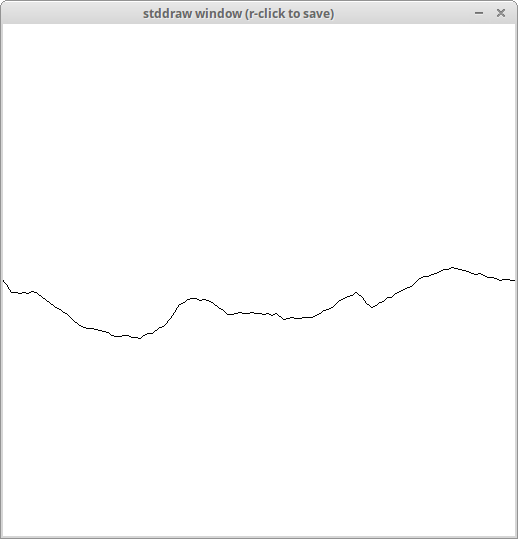
\includegraphics[scale=0.15]{figures/brownian1.png}}
\end{minipage}

\pause
\smallskip

\begin{minipage}{160pt}
\begin{lstlisting}[language={}]
$ python3 brownian.py .5
\end{lstlisting}
\end{minipage}%
\begin{minipage}{140pt}
\hfill \visible<3->{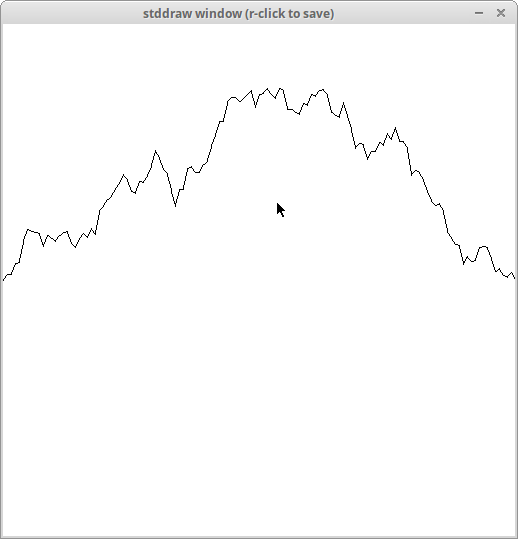
\includegraphics[scale=0.15]{figures/brownian2.png}}
\end{minipage}

\pause
\smallskip

\begin{minipage}{160pt}
\begin{lstlisting}[language={}]
$ python3 brownian.py .05
\end{lstlisting}
\end{minipage}%
\begin{minipage}{140pt}
\hfill \visible<4->{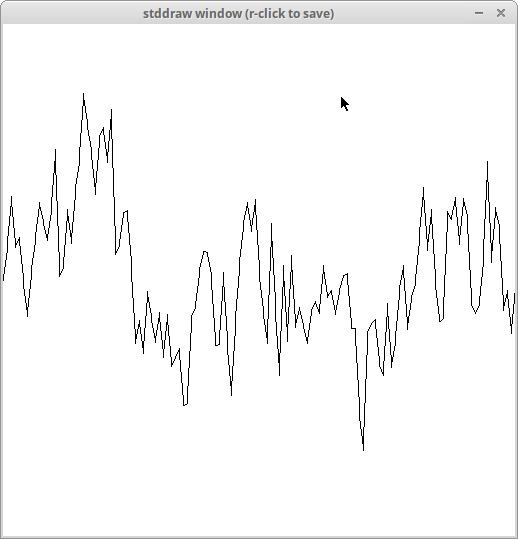
\includegraphics[scale=0.15]{figures/brownian3.png}}
\end{minipage}
\end{frame}

\section{Pitfalls}
\begin{frame}[fragile]
\pause

Missing base case
\begin{lstlisting}[language=Python]
def harmonic(n):
    return 1 / n + harmonic(n - 1)
\end{lstlisting}

\pause
\bigskip

Recursion does not address smaller subproblems
\begin{lstlisting}[language=Python]
def harmonic(n):
    if n == 1:
        return 1
    return 1 / n + harmonic(n)
\end{lstlisting}

\pause
\bigskip

\begin{minipage}{150pt}
Recursion addresses overlapping subproblems; for example, computing $N$th Fibonacci number

\begin{lstlisting}[language=Java]
def f(n):
    if n == 0 or n == 1:
        return n
    return f(n - 1) + f(n - 2)  
\end{lstlisting}
\end{minipage}
\begin{minipage}{150pt}
\begin{center}
Call trace for \lstinline{f(5)}

\smallskip

\visible<4->{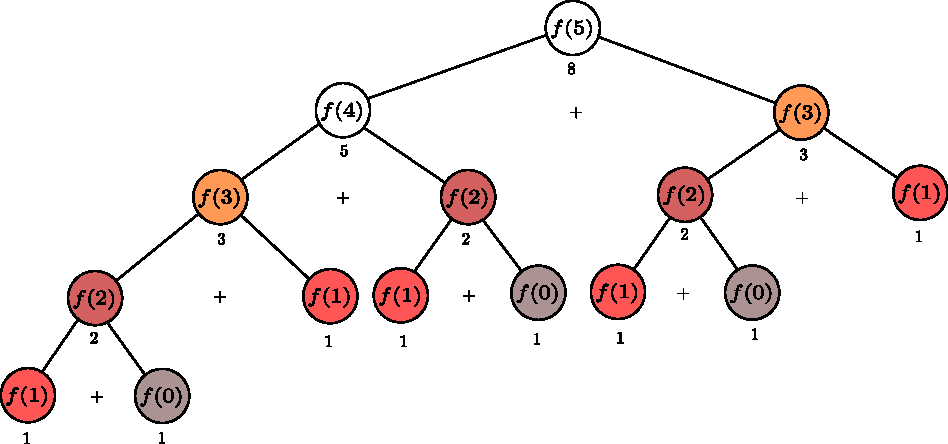
\includegraphics[scale=0.35]{figures/fib_trace.pdf}}
\end{center}
\end{minipage}

\pause
\bigskip

If a function calls itself recursively an excessive number of times before returning, the memory required by Python to keep track of the recursive calls may be prohibitive, resulting in a runtime error
\end{frame}
\end{document}
